% Anonymous RA-L initial-submission draft. Compile twice with pdflatex.
% The bibliography is inline. The source archive includes ieeeconf.cls and the figure.
% Complete the evaluation before submitting. Protocol choices are prospective.
\documentclass[letterpaper,10pt,conference]{ieeeconf}
\overrideIEEEmargins
\usepackage{amsmath,amssymb,graphicx,booktabs,url}
\title{\LARGE\bf BimanualPFN: Compositional Generalization in Bimanual Manipulation with Prior-Data Fitted Networks}
\author{\mbox{}}
\pdfinfo{/Title (BimanualPFN: Compositional Generalization in Bimanual Manipulation with Prior-Data Fitted Networks) /Author ()}
\begin{document}
\maketitle
\thispagestyle{empty}\pagestyle{empty}
\begin{abstract}
A three-object shelf-restocking demonstration leaves an important decision unobserved. After the third placement in a new scene, should the robot stop or reach for a fourth object? We propose BimanualPFN, a demonstration-conditioned prior-data fitted network for inferring how a bimanual task extends to a different scene. An analytic generator pairs episodes that share a manipulation rule and a compositional rule while varying object counts, layouts, and arm configurations. A time-indexed table represents each gripper, object, and target with the same position-and-quaternion format. Semantic column headers identify what each pose describes. Given one completed demonstration and the observed query history, the network predicts two synchronized columns of future wrist poses. A visual action policy uses these poses, images, and proprioception to generate executable commands. We specify paired tests of task selection, stopping, and handover timing with ACT and GR00T executors. Preliminary measurements with an earlier event predictor motivate these tests. Closed-loop performance of the proposed pose-window model remains to be measured.
\end{abstract}
\noindent\textbf{\textit{Index Terms}}---Learning from Demonstration, Bimanual Manipulation.

\section{Introduction}
A demonstration can specify which objects belong on a shelf, the order in which to move them, and how two arms should share the work. Consider a demonstrator who restocks three cans, passing each from one gripper to the other. With two eligible cans, reaching for a third could disturb the completed arrangement. With four eligible cans, the robot must initiate a transfer that has no counterpart at the same time in the demonstration. Each handover also imposes a timing constraint. Even a correctly selected object can fall if the giver opens while the receiver is still approaching.

A single demonstration rarely identifies the task uniquely. Moving three cans is consistent with transferring every can, moving every object, and stopping after three transfers. Including distractors helps distinguish the first two interpretations. Distinguishing a fixed repetition count from an instruction to continue until a set is exhausted may require another observation or a prior preference. We ask what a synthetic prior contributes when a visual policy must act on one such example. The setting permits pretraining on many synthetic tasks and fitting the executor on action-labelled source demonstrations. At deployment, one completed demonstration provides the target composition, and the models' weights are fixed.

Human behavioral studies test compositionality by asking whether familiar components can be reused in an unfamiliar combination~\cite{luettgau}. We adopt this criterion by withholding a manipulation--selection pairing while retaining each constituent in training. BimanualPFN learns to fill two missing wrist-pose columns in a new scene. Each synthetic training item links a support demonstration to an independent query episode generated under the same rule. The support shows how entities and wrists move together. The query determines which entities exist now and which operation remains feasible. A frozen network predicts a short pose window for both wrists. A visual policy refines that window into robot commands (Fig.~\ref{fig:system}).

Our contributions are a simulator-free prior that separates bimanual manipulation from selection, ordering, and repetition, a homogeneous table interface for predicting coupled poses across variable entity sets, and a paired evaluation that tests whether changing the demonstration changes the completed task. An earlier event predictor could read a compaction instruction offline, while its shelf experiments gave weaker evidence of a gain in completed tasks. Section~\ref{sec:pilot} reports these observations and motivates an evaluation that measures inference and execution separately.

\begin{figure*}[t]
\centering
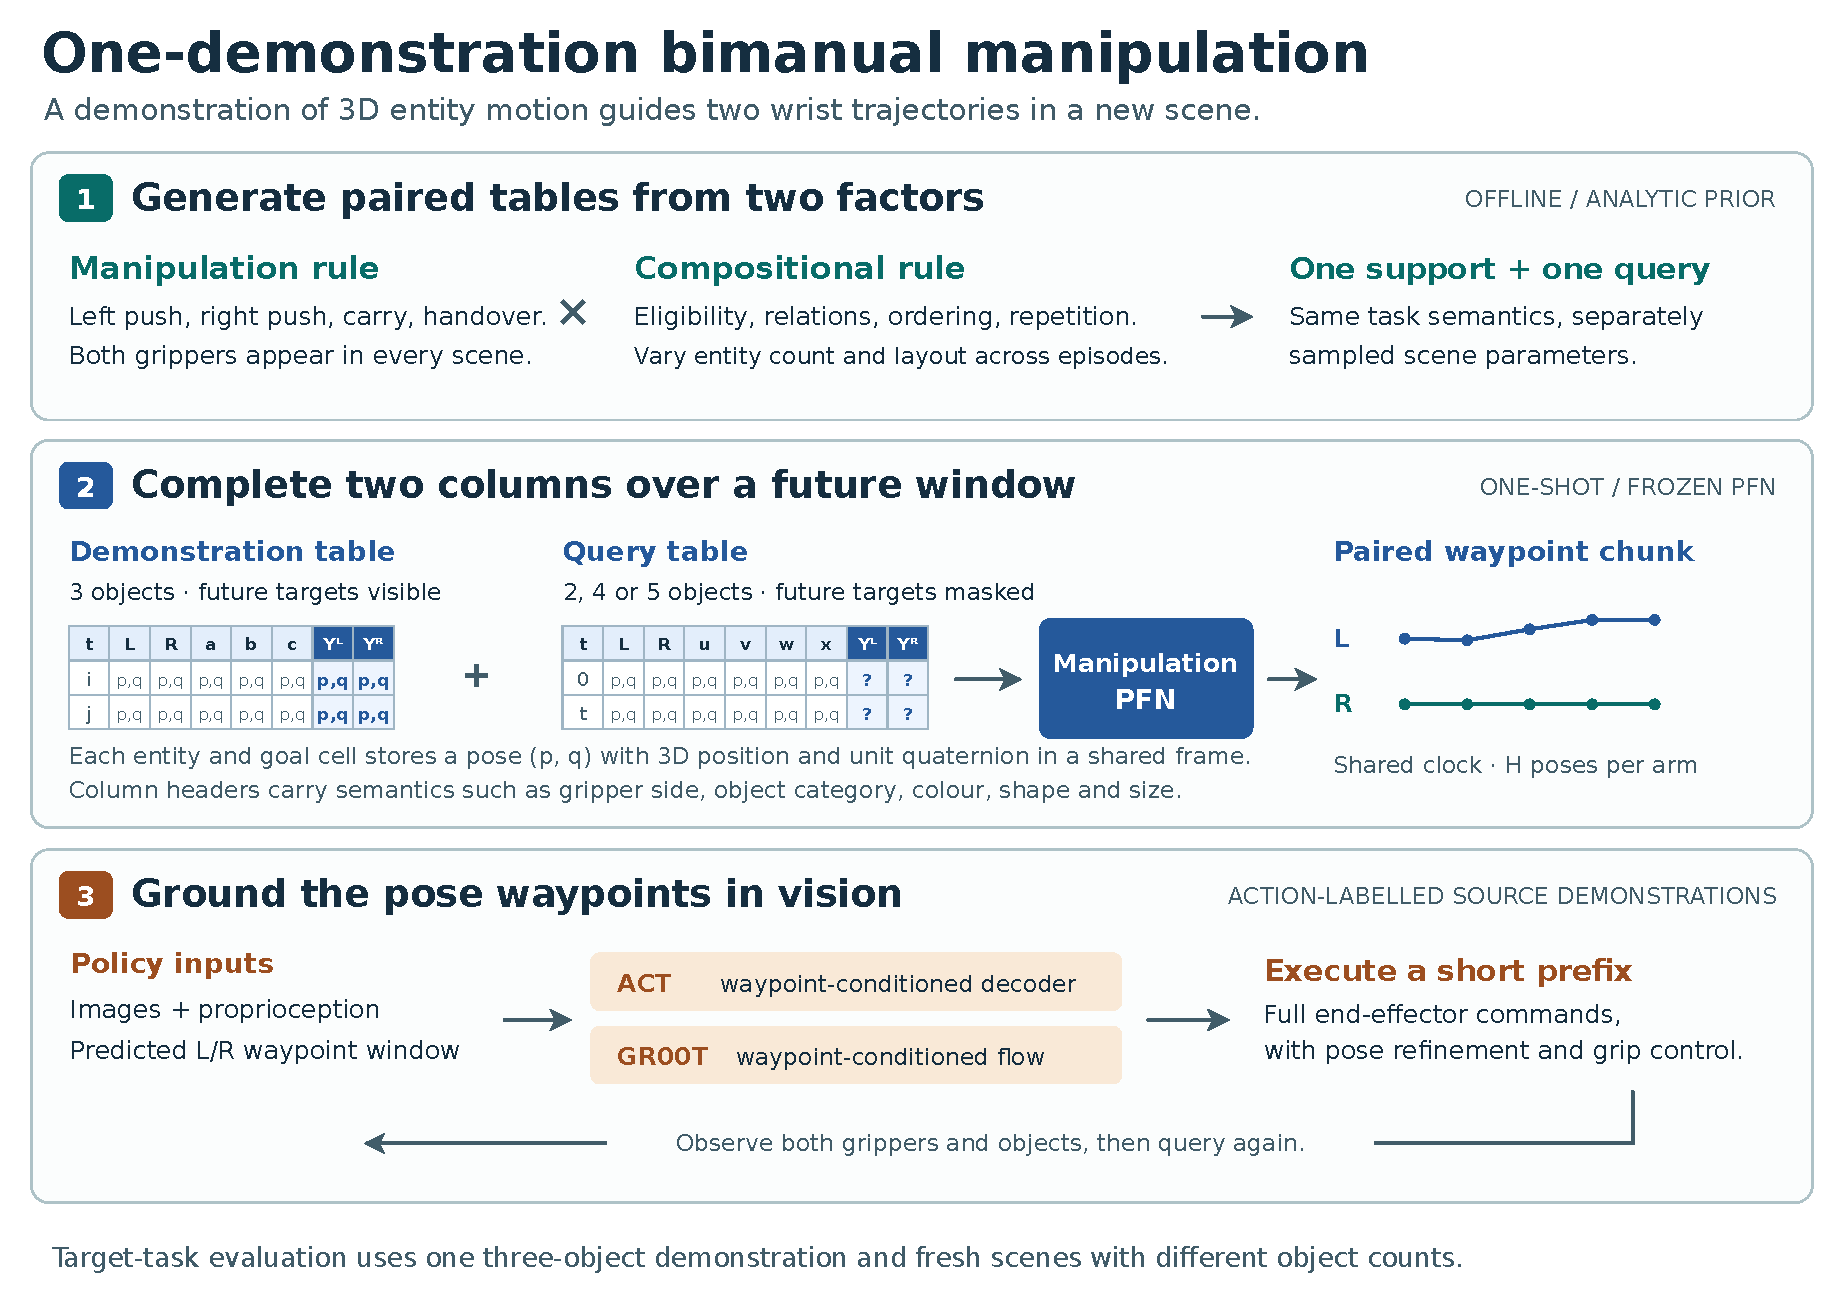
\includegraphics[width=.91\textwidth]{figures/OCT_VLA_One_Demonstration.pdf}
\caption{BimanualPFN overview. Letters denote episode-local entity tracks. Each observed or target cell stores a position and a unit quaternion. The two query target columns are masked. The PFN predicts both wrists on one clock, and a visual policy executes a prefix before observing the scene again. The traces illustrate temporal alignment.}
\label{fig:system}
\end{figure*}

\section{Related Work}
\textit{Imitation from a demonstration.}
Instant Policy learns in-context imitation by graph diffusion over demonstrations, observations, and actions. It uses simulated pseudo-demonstrations to train a policy that can acquire a task from one or two examples~\cite{instant}. DemoGen transforms a human demonstration and its 3D observations into training examples for other object configurations, including bimanual tasks~\cite{demogen}. RICL adds in-context adaptation to pretrained vision-language-action models (VLAs) using robot demonstrations~\cite{ricl}, and StellaVLA conditions a VLA on a structured description extracted from a demonstration~\cite{stella}. These works establish precedents for both structured demonstration context and synthetic training. We study whether generalization benefits from independent variation of primitive, relational rule, and entity count during pretraining. A direct demonstration-conditioned policy and an equal-budget ablation of this variation are therefore central comparisons.

\textit{Prior-data fitted networks.}
A PFN trains on datasets sampled from a task prior to approximate predictions conditioned on observed examples~\cite{pfn}. TabPFN applies this principle to tabular data and supports distributional regression~\cite{tabpfn}. Here rows are correlated time steps, columns carry entity tracks, and the target comprises two trajectories on $\mathrm{SE}(3)$. An episodic prior over manipulation tasks supplies the analogue of a prior over tabular prediction problems. We adopt the predictive training principle. The pose decoder estimates a conditional trajectory and makes no assumption of calibrated posterior uncertainty.

\textit{Visual execution under distribution shift.}
ACT predicts chunks of actions for fine bimanual control~\cite{act}. GR00T N1.7 uses a flow-matching transformer for action generation conditioned on observations~\cite{groot}. These executors let us evaluate the same synthetic pose prior with two control architectures. RoboMME-Plus varies object count alongside motion, occlusion, and demonstration history~\cite{robomme}. Its shifts motivate a controlled test of count transfer in which perceptual degradation and contact failures can be scored separately.

\section{Problem Formulation}
Let $D$ be a completed support demonstration for a latent task $r$, and let $Q_{\le t}$ contain the observed history of a fresh scene. Both grippers appear in every episode, including intervals when one is idle. Each entity $e$ has a pose $T_{t,e}=(p_{t,e},q_{t,e})$, where $p_{t,e}\in\mathbb R^3$ and $q_{t,e}$ is a unit quaternion. All poses are expressed in a shared calibrated workcell frame. The static column header $s_e$ describes the entity using available attributes such as category, colour, size, shape, or gripper side. Time is the row index. A track is consistent within an episode. Different episodes can have different numbers of objects and different column orders.

The two goal columns store commanded poses of the left and right wrists in exactly the same seven-value representation. The prediction at time $t$ is
\begin{equation}
Y_t^\star =
\big((T^{L,\mathrm{cmd}}_{t+h}, T^{R,\mathrm{cmd}}_{t+h})\big)_{h=1}^{H}.
\label{eq:window}
\end{equation}
This $H\times2\times7$ chunk contains geometry and timing for both arms. Gripper aperture remains part of the executor's action space. The support exposes the complete pose and command tracks. The query exposes observed entity history through $t$. Future query observations and commands are withheld, including interpolation or smoothing that would use future measurements. Masks also distinguish padded objects and missing observations. Cadence and command timestamps must agree across synthetic trajectories and robot recordings.

Test-time adaptation consists of encoding the support once and using it throughout a rollout. The method assumes calibrated wrist poses, tracked object poses, and observable semantics. An evaluation using simulator state measures inference under privileged perception. Estimating the same quantities during a physical handover adds calibration and occlusion errors, so perception source must be reported with each result.

\section{BimanualPFN}
\subsection{An analytic prior over episode pairs}
Draw a manipulation rule $m$ and a compositional rule $c$ from a distribution over feasible combinations. Independently sample support and query scene parameters $\xi_D,\xi_Q$ conditional on those rules. With analytic generator $\mathcal G$, the paired episodes are
\begin{equation}
D=\mathcal G(m,c,\xi_D),\qquad Q=\mathcal G(m,c,\xi_Q).
\end{equation}
The shared rule specifies the task. Its two instantiations determine which objects are present and how the grippers must move. For instance, the same rule can transfer eligible cans in their demonstrated order until the eligible set is empty. The generator updates object and wrist poses after each operation and samples query prefixes during execution. The resulting labels are analytic trajectories without a physics simulation.

\textit{Manipulation.}
For a push, sample an object frame, a desired push direction, and a contact point on the rear surface. Use the acting arm's tool transform, feasible workspace, and initial pose to construct its approach. Both left- and right-arm pushes occur. The other arm receives a stationary or clearance trajectory. For transport, sample a grasp transform and preserve the relative wrist--object pose over the attached interval. For handover, sample feasible giver and receiver grasp frames and a shared interval during which the giver holds while the receiver approaches and acquires the object. Vary the arm assignments and timing. Sample intermediate positions and interpolate orientations along the short quaternion arc on a fixed physical clock. These rules specify intended contact geometry and order. Robot demonstrations supply the evidence for contact-rich execution.

\textit{Reactive coordination.}
We branch an analytic handover into punctual and delayed receiver approaches. Once the delay is observable, the giver extends its hold and the receiver continues its approach. Both targets are recomputed from the observed exchange state. We mirror giver and receiver roles and include undisturbed controls (Fig.~\ref{fig:atlas}). An independent observation model applies temporally contiguous gaps or delays to the query object tracks. The PFN receives measurement validity and age when available, while proprioception supplies both wrist poses. During an unresolved occlusion, the target can specify a hold until the object becomes observable again.

\begin{figure*}[t]
\centering
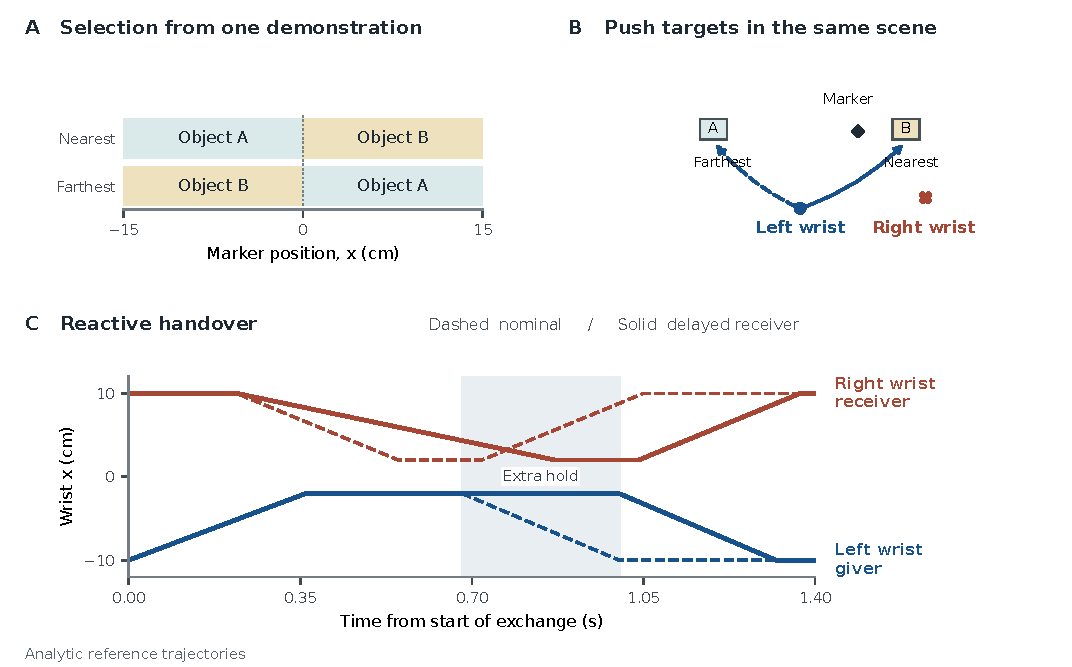
\includegraphics[width=.92\textwidth]{figures/BimanualPFN_Validation_Atlas.pdf}
\caption{Analytic validation examples. The first two panels show how changing the demonstration selects a different push target for the same left wrist and scene. The third shows paired wrist targets during a delayed handover. Dashed paths denote the nominal exchange. All traces are generated references.}
\label{fig:atlas}
\end{figure*}

\textit{Composition.}
Vary eligibility predicates, spatial or semantic references, ordering, and repetition independently of geometry where feasible. Consider two supports that indicate either a red object or the nearest object to a tray. One query scene can make these two selections disagree. Holding the scene fixed makes the demonstration necessary. Conversely, adding a distractor under the same rule can leave the intended wrist paths unchanged. Permute entire object columns with their semantic headers and masks. Vary dwell times, initial arm poses, and support layouts within each rule to remove simple timing and slot shortcuts. The task specifies whether ordering matters. Left-to-right is one possible demonstrated ordering.

\subsection{Encoding and predicting paired trajectories}
A shared encoder embeds a pose together with its column-header embedding. Within-row attention exchanges information between wrists, objects, and the two goal cells. Within-episode temporal attention follows each track. Across episodes, the query reads encoded support rows via their aligned gripper and goal columns. Object information reaches those columns through within-row attention. This preserves both arm identities across episodes without assuming that the third object in a demonstration matches the third query object. The support representation can be cached. Query attention may retrieve a grasp configuration early and the giver--receiver relationship later.

We propose a joint decoder with a query for each arm and horizon, permitting the two arms to attend to each other. Let $R_t^a$ be the measured rotation of arm $a$. For each future horizon the decoder predicts a translation relative to the current wrist in workcell axes and a rotation increment in the current wrist frame. Absolute poses are reconstructed as
\begin{equation}
\widehat p^a_{t+h}=p^a_t+\widehat{\Delta p}^a_h,\qquad
\widehat R^a_{t+h}=R^a_t\,\widehat{\Delta R}^a_h .
\end{equation}
Every horizon uses the same measured anchor. All external inputs and outputs carry normalized quaternions. Enforce temporal sign continuity on input tracks to avoid a representation jump between equivalent $q$ and $-q$.

The generator defines a distribution over tasks, support episodes and query prefixes. Pretraining minimizes the expected window loss over fresh draws from this distribution. A training example therefore contributes supervision for predicting one episode given evidence from another. Its valid arm--horizon pairs $\mathcal V$ contribute
\begin{align}
\mathcal L=\frac{1}{|\mathcal V|}\sum_{(a,h)\in\mathcal V}
\Big[&\rho\big((\widehat p^a_{t+h}-p^{a,\star}_{t+h})/\ell\big)\nonumber\\
&+\lambda_R\big(1-\langle\widehat q^a_{t+h},q^{a,\star}_{t+h}\rangle^2\big)\Big].
\label{eq:loss}
\end{align}
Here $\rho$ sums coordinate-wise Huber penalties, $\ell$ is a fixed workspace length, and $\lambda_R$ controls the rotation penalty. The squared inner product respects quaternion sign equivalence. Mask targets after episode end. Sample moving, holding, and contact-transition windows explicitly, since a predictor can otherwise lower its average error by keeping both arms still. A deterministic estimator can average incompatible paths for ambiguous supports. These cases warrant separate analysis.

\subsection{Learning the visual executor}
The executor $\pi_\phi$ receives images $I_t$, proprioceptive history $u_{\le t}$ including aperture, and $\widehat Y_t=f_\theta(D,Q_{\le t})$. It produces a chunk of full end-effector commands for both arms. For ACT, arm- and time-labelled pose embeddings enter the observation memory read by the action queries. For GR00T, we propose a separate cross-attention branch for the pose embeddings in the action head. The flow starts from its usual Gaussian source and is conditioned on the pose window during generation. In each case the policy executes a short prefix and obtains a new scene observation before the next prediction.

At each training step we sample two independent, task-compatible source recordings: one complete support and one query. For each sampled query time $t$, the frozen PFN reads the last $L$ observed rows through $t$ and predicts the next $H$ paired wrist poses. Future query rows supply loss targets only. The executor receives this predicted chunk, synchronized head, left-wrist and right-wrist images at $t$ (optionally recent frames), and causal proprioception. It predicts workcell translation corrections, local rotation increments and gripper commands. For predicted wrist pose $(\hat p,\hat R)$, the executed target is $(\hat p+\delta p,\hat R\exp([\delta\omega]_\times))$. Expert query commands supervise these corrections at matching timestamps. ACT regresses residual chunks, and GR00T uses conditional flow matching in residual action space. We resample supports and times across training and fix one support per test rollout.


\section{Preliminary Evidence and Its Scope}
\label{sec:pilot}
An earlier time-row model predicted discrete events and keyframe targets. Table~\ref{tab:pilot} summarizes its offline compaction test. Each item pairs two programs whose desired decisions differ only in whether an object should be compacted. A pair scores one only when both predictions are correct. The one-seed measurements show substantial sensitivity to the support and a smaller gap on held-out compositions. These scores measure the predecessor's decision to compact.
\begin{table}[t]
\centering
\caption{Earlier event predictor, one training seed. Fraction of conflict pairs with both compaction decisions correct.}
\label{tab:pilot}
\begin{tabular}{lrrr}
\toprule
Synthetic split & Pairs & Correct support & Shuffled\\
\midrule
Training-rule distribution & 66 & .82 & .02\\
Held-out composition & 104 & .83 & .40\\
Shelf family & 284 & .85 & .05\\
\bottomrule
\end{tabular}
\end{table}

Earlier closed-loop shelf tests gave a different picture. Across three training seeds and 20 four-object scene resets per seed, a calibrated keyframe prior achieved more transfers than a scene-conditioned GR00T baseline on 28 matched rollouts and fewer on 12. Full-task successes were 6/60 with that prior and 5/60 with scene conditioning. These descriptive counts share scene layouts across training seeds. They motivate scoring preservation and final completion separately from progress. Neither experiment used the homogeneous pose-window target in Eq.~\eqref{eq:window}. End-to-end performance of the new model is open.
% Author-side provenance: Alonso94/OCT_VLA, pfn-vla, paper/5_time_row_pfn_design.md,
% Sec. 12.2, and paper/3_pfn_vla_interface.md, the three-seed shelf study.
% Check raw run IDs and denominators before final submission.

\section{Experimental Design}
\subsection{Splits and primary endpoint}
The proposed primary task is dual-Franka shelf restocking. Each target support demonstrates three objects. Fresh scenes contain two, three, or four eligible objects for the primary count test, with a separate distractor condition. We reserve five objects as an extrapolation stress test, subject to shelf capacity and expert feasibility on the same layouts. The proposed split allows at most four eligible objects in synthetic pretraining and three in source shelf recordings. Under this split, four tests transfer beyond the robot data and target support. Five also exceeds the synthetic range. A separate split withholds a complete manipulation--composition pair from synthetic training and source execution data while keeping its constituent rules available. Freeze all choices on development tasks, including thresholds, support selection and checkpoint selection. Claims about unseen tasks apply to the data under experimental control. The full training data of a pretrained VLA may be only partly auditable.

Primary success is measured per reset. All eligible objects must occupy their assigned regions in the demonstrated order when the rule specifies one, distractors must remain undisturbed, and placements must stay stable over a prespecified interval. On a two-object scene we require the policy to settle after the second placement. At higher counts we record whether it initiates and completes transfers beyond the support count. A no-motion period midway through a handover cannot establish completion. The evaluator checks predicates from the scene state. No oracle stopping signal is passed to the policy. Freeze the dwell interval, displacement tolerance, and timeout on development scenes before scoring either method.

A second task tests handover with giver and receiver roles varied across supports. Score whether the receiver acquires the object before giver release, retains it after release, and delivers it to its destination. Score the overall endpoint on all attempted resets. A phase-conditioned breakdown locates the first failed stage. An independent contact or attachment signal is preferable for scoring acquisition. If only aperture and motion are available, validate the proxy on annotated transfers.

\subsection{Comparisons that locate the failure}
\textit{Can the executor follow a pose window?}
Use an expert that computes a feasible pose window from the current rollout state and a specified rule. First test ACT, then use the same scenes for GR00T. Recorded future commands are useful for checking offline timing and frame conventions. Once a policy departs from a recording, the online oracle must recompute its window. Compare accurate windows, feasible counterfactual windows, and frozen-PFN predictions with identical executor weights. This intervention measures the executor's sensitivity to its conditioning. Its success rate need not bound other controllers.

\textit{Does the demonstration specify the task?}
Reset the same feasible scene under two supports whose rules require different first objects. Use independent support layouts and keep the language input, initial robot state and policy randomness fixed. Measure the fraction of pairs for which \emph{both} first pickups succeed on their respective objects. A fixed preference can score well on one direction but fails the paired test. Log the first intended approach from the predicted pose window and the first object actually acquired, using a prespecified association radius and marking ambiguous approaches separately. Hold count fixed for this experiment to isolate support sensitivity from repetition.

\textit{Does the factorized prior contribute?}
For each backbone compare scene conditioning alone, direct conditioning on the same demonstration table, and BimanualPFN. Give all arms the same available scene information and match source robot data, command normalization, backbone adaptation and action horizon. The direct-support arm controls for access to task evidence. A matched pose predictor trained on source data alone tests the contribution of synthetic pretraining. An equal-budget synthetic ablation constrains support and query counts to be equal while keeping their marginal count distributions. This isolates learning across count mismatches. A nominal-only prior tests the contribution of the reactive branches. A second ablation removes coupled handovers during synthetic training while retaining arm-specific pushes and carries, matching marginal movement and training budget as closely as possible. Report residual differences in task coverage. On handover, report coordinated retention alongside per-arm trajectory error.

\textit{Can visual feedback recover a faulty plan?}
We occlude the target in the head view during approach while verifying that a wrist camera still sees it. Starting from the same scene and briefly holding the PFN window fixed, we compare live wrist images with withholding the informative wrist view(s). We repeat at exchange with an occluded receiving-wrist view, and then restore normal PFN updates. We score signed correction, acquisition, retention and complete recovery. A missing detection preserves the expert command when the world is unchanged. A physical drop requires new expert commands from the disturbed state. We report how the scene table was obtained and score all-view occlusion separately after reacquisition.

\textit{How much can geometric replay explain?}
Retarget demonstrated wrist trajectories to matched object frames and repeat demonstrated segments over eligible objects. Give this baseline the same observable semantic attributes and state how segments and correspondences are assigned. If an oracle supplies eligibility or segmentation, label that comparison privileged. On a shelf where retargeting and repetition already solve the task, this baseline places the learned prior's contribution in perspective.

\subsection{Analysis and reporting}
Report successes and attempted resets for each count and backbone, with the paired difference from the direct-support baseline. Repeat over independent single demonstrations, layouts, and training seeds. Reuse the same supports and layouts across methods, retaining both members of each matched pair. Report seed-level outcomes and intervals that respect the crossed sampling of supports and layouts. Multiple objects within one rollout and repeated trials of a single checkpoint are dependent observations. Stratify complete success by count, because a fixed error rate per transfer can reduce success mechanically as the task grows.

For offline tests, report translation error in physical units, sign-invariant angular error in degrees, moving-arm error, idle-arm drift, and the relative wrist-transform error during handover. For closed-loop diagnosis, overlay the predicted and measured wrists in paired rollout filmstrips and mark the first approach, pickup, release, and stable placement. Different predicted approaches followed by identical robot motion indicate weak executor conditioning. Rule-consistent first pickups followed by drops point to execution failures. These observations supplement the primary endpoint of complete task success.
% Before submission: insert actual budgets, seeds, independent supports/layouts,
% control cadence, H, prefix length, calibration conventions, observation modality,
% train/test manifests and measured outcomes. Update Abstract and Conclusion.

\section{Discussion and Limitations}
The pose interface makes its information limits explicit. Two nearly identical wrist poses may precede opposite aperture commands. Images and recent gripper state may resolve this ambiguity. The oracle-window comparison tests whether the available observations suffice. A unit quaternion also depends on a chosen object frame. A rotationally symmetric can has multiple visually equivalent orientations. Consistent annotations or a symmetry-aware observation encoder are needed wherever this ambiguity affects the input. Wrist error is evaluated in the calibrated physical tool frame.

The analytic generator defines plausible geometric interactions. It cannot establish that a real grasp resists slip or that a controller recovers after a drop. Count shifts can also introduce crowding and increase the number of opportunities for failure. A useful control varies eligible count at fixed physical count, then varies total clutter at fixed eligibility. Finally, identical demonstrations can support incompatible rules. The intended scope of one-shot adaptation is the set of behaviours distinguishable from the support under the specified prior.

\section{Conclusion}
BimanualPFN formulates one-demonstration bimanual manipulation as completion of two synchronized pose columns. A synthetic task prior exposes the predictor to rules over changing entity sets, while robot demonstrations train a visual executor. The decisive test is whether a single policy can stop at two, continue beyond three, and preserve the demonstrated arm coordination on a held-out task.

\begin{thebibliography}{10}
\bibitem{luettgau} L. Luettgau \emph{et al.}, ``Decomposing dynamical subprocesses for compositional generalization,'' \emph{Proc. Natl. Acad. Sci. USA}, vol.~121, no.~46, e2408134121, 2024.

\bibitem{instant} V. Vosylius and E. Johns, ``Instant Policy: In-context imitation learning via graph diffusion,'' in \emph{Proc. ICLR}, 2025.
\bibitem{demogen} Z. Xue, S. Deng, Z. Chen, Y. Wang, Z. Yuan, and H. Xu, ``DemoGen: Synthetic demonstration generation for data-efficient visuomotor policy learning,'' arXiv:2502.16932, 2025.
\bibitem{ricl} K. Sridhar \emph{et al.}, ``RICL: Adding in-context adaptability to pre-trained vision-language-action models,'' in \emph{Proc. CoRL}, PMLR, vol.~305, pp.~5022--5038, 2025.
\bibitem{stella} S. Xu \emph{et al.}, ``StellaVLA: In-context structured demonstration for generalizable vision-language-action models,'' arXiv:2608.11671, 2026.
\bibitem{pfn} S. M\"uller, N. Hollmann, S. Pineda Arango, J. Grabocka, and F. Hutter, ``Transformers can do Bayesian inference,'' in \emph{Proc. ICLR}, 2022.
\bibitem{tabpfn} N. Hollmann \emph{et al.}, ``Accurate predictions on small data with a tabular foundation model,'' \emph{Nature}, vol.~637, pp.~319--326, 2025.
\bibitem{act} T. Z. Zhao, V. Kumar, S. Levine, and C. Finn, ``Learning fine-grained bimanual manipulation with low-cost hardware,'' in \emph{Proc. Robotics: Science and Systems}, 2023.
\bibitem{groot} NVIDIA, \emph{GR00T-N1.7-3B model card}, 2026. [Online]. Available: \url{https://huggingface.co/nvidia/GR00T-N1.7-3B}
\bibitem{robomme} Y. Dai, H. Fu, Y. Liu, C. Finn, N. Fazeli, and J. Chai, \emph{RoboMME-Plus: Benchmarking memory generalization for robot policies}, 2026. [Online]. Available: \url{https://robomme.github.io/plus.html}
\end{thebibliography}
\end{document}

